\documentclass{beamer}
\usepackage{amsthm}
\usepackage{amsmath}
\usepackage{amsfonts}
\usepackage{amssymb}
\usepackage{epic}
\usepackage{graphicx}
\usepackage{epstopdf}
\usepackage{multirow}
\usetheme{Berlin}
\usecolortheme{seahorse}
\usepackage{multicol}



\newtheorem{question}{Question}[section] 

\title{Project 2: The Plight of the Late Flight}



\author{Andrew Bernath, Heather Kitada, Ethan Edwards}



\institute{Oregon State University}



\begin{document}

\begin{frame}
\titlepage
\end{frame}


\begin{frame}
\begin{center} 
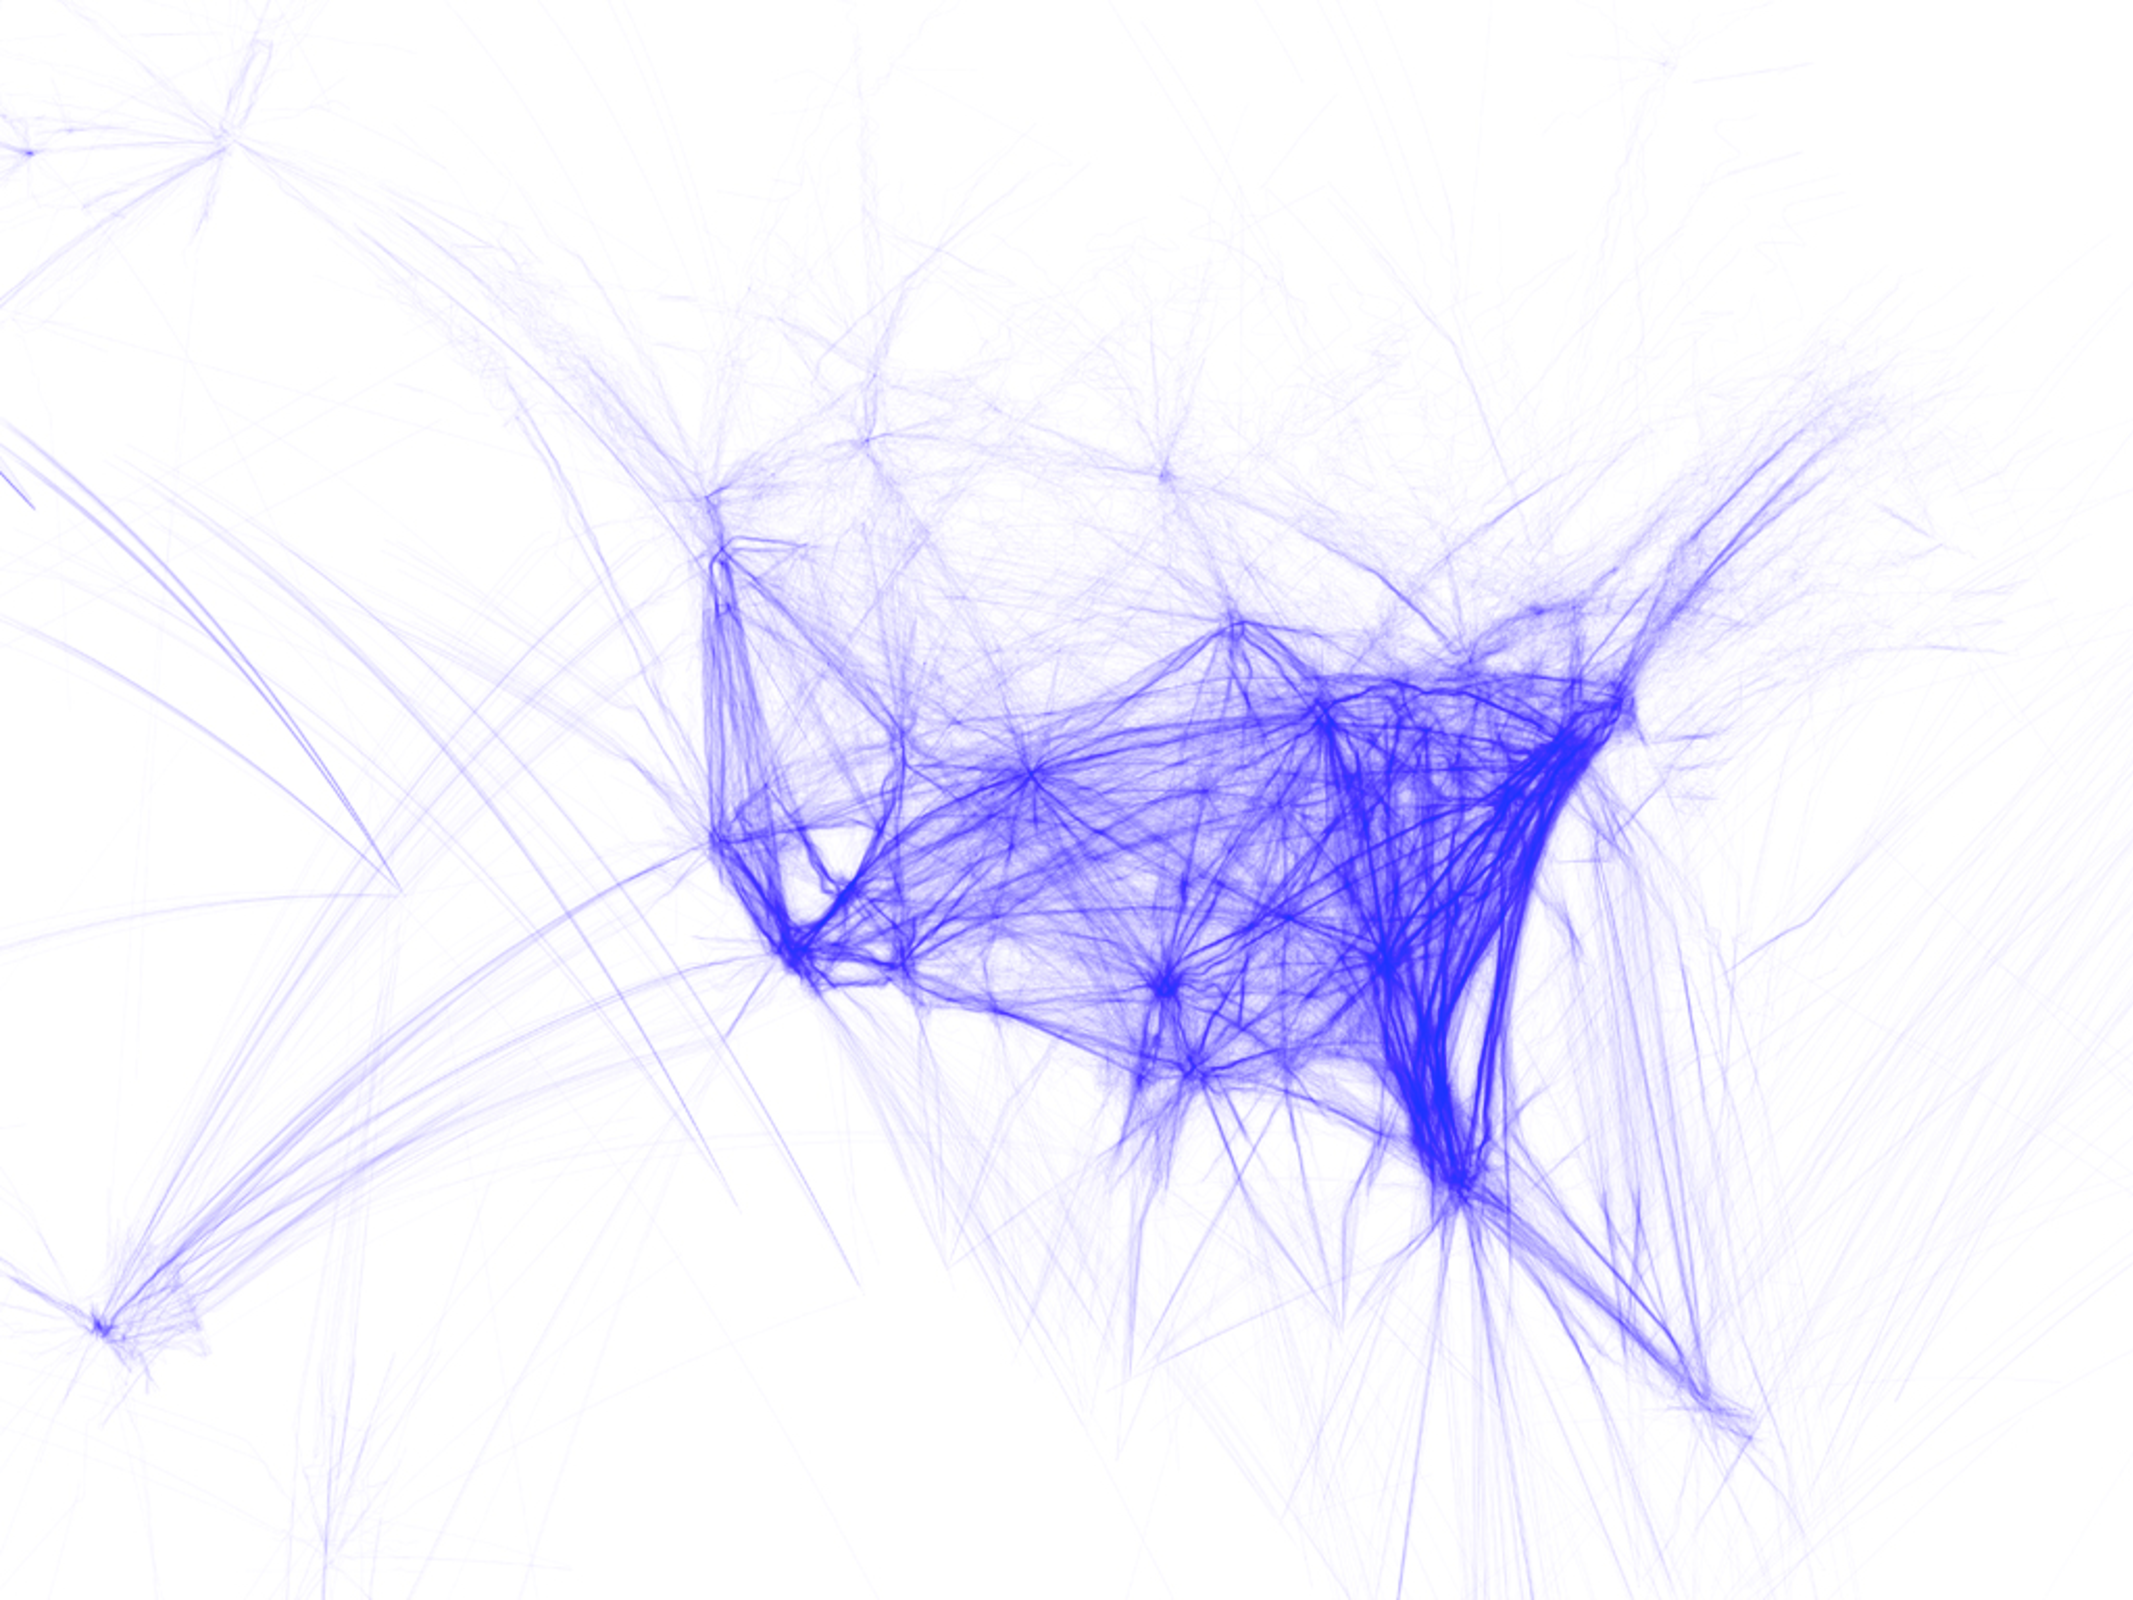
\includegraphics[width=.9 \textwidth]{airtraffic}
\end{center}
\tiny{Image credit: Aaron Koblin}

\end{frame}

\begin{frame}{\contentsname}
\begin{multicols}{2}
\tableofcontents
\end{multicols}
\end{frame}

\section{Overview and Question of Interest}
\begin{frame}
\frametitle{Overview}
\begin{itemize}
\item Data: Bureau of Transportation Statistics (BTS)
\item Last 25 years 
\item 30 Unique carriers 
\item 376 Unique origins 
\end{itemize}

\end{frame}

\subsection{Question of Interest}
\begin{frame}
\frametitle{Question of Interest}

Are there any airlines that have shown consistent improvement in delays, across the entire country, over the 25 years of flight data?

\end{frame}

\subsection{Choosing A Metric}
\begin{frame}
\frametitle{How do we define "improvement" in delay?}
\begin{itemize}
\item Improvement is defined as negative change in delay time, where delay can be measured using the following metrics:

\begin{itemize}
\item Arrival delay 
\begin{itemize}
\item What customers care about
\end{itemize}

OR
\item Carrier + Late Aircraft delays 
\begin{itemize}
\item What carriers are able to control 
\end{itemize}
\end{itemize}
\item Overall improvement metric = Median change in mean delay 
\end{itemize}

\end{frame}

\subsection{Narrowing Scope}
\begin{frame}
\frametitle{Narrowing Scope}
\begin{itemize}
\item Ran all airlines and years 
\item Only kept airlines with 10+ years of service 
\begin{itemize}
\item 10+ is enough to discern a pattern
\end{itemize}
\item Aggregating to create yearly averages 
\begin{itemize}
\item Average over seasonal effects to compare year to year 
\end{itemize}
\end{itemize}

\end{frame}



\section{Population-Based Findings}
\begin{frame}
\frametitle{Population-Based Findings}
\begin{center} 
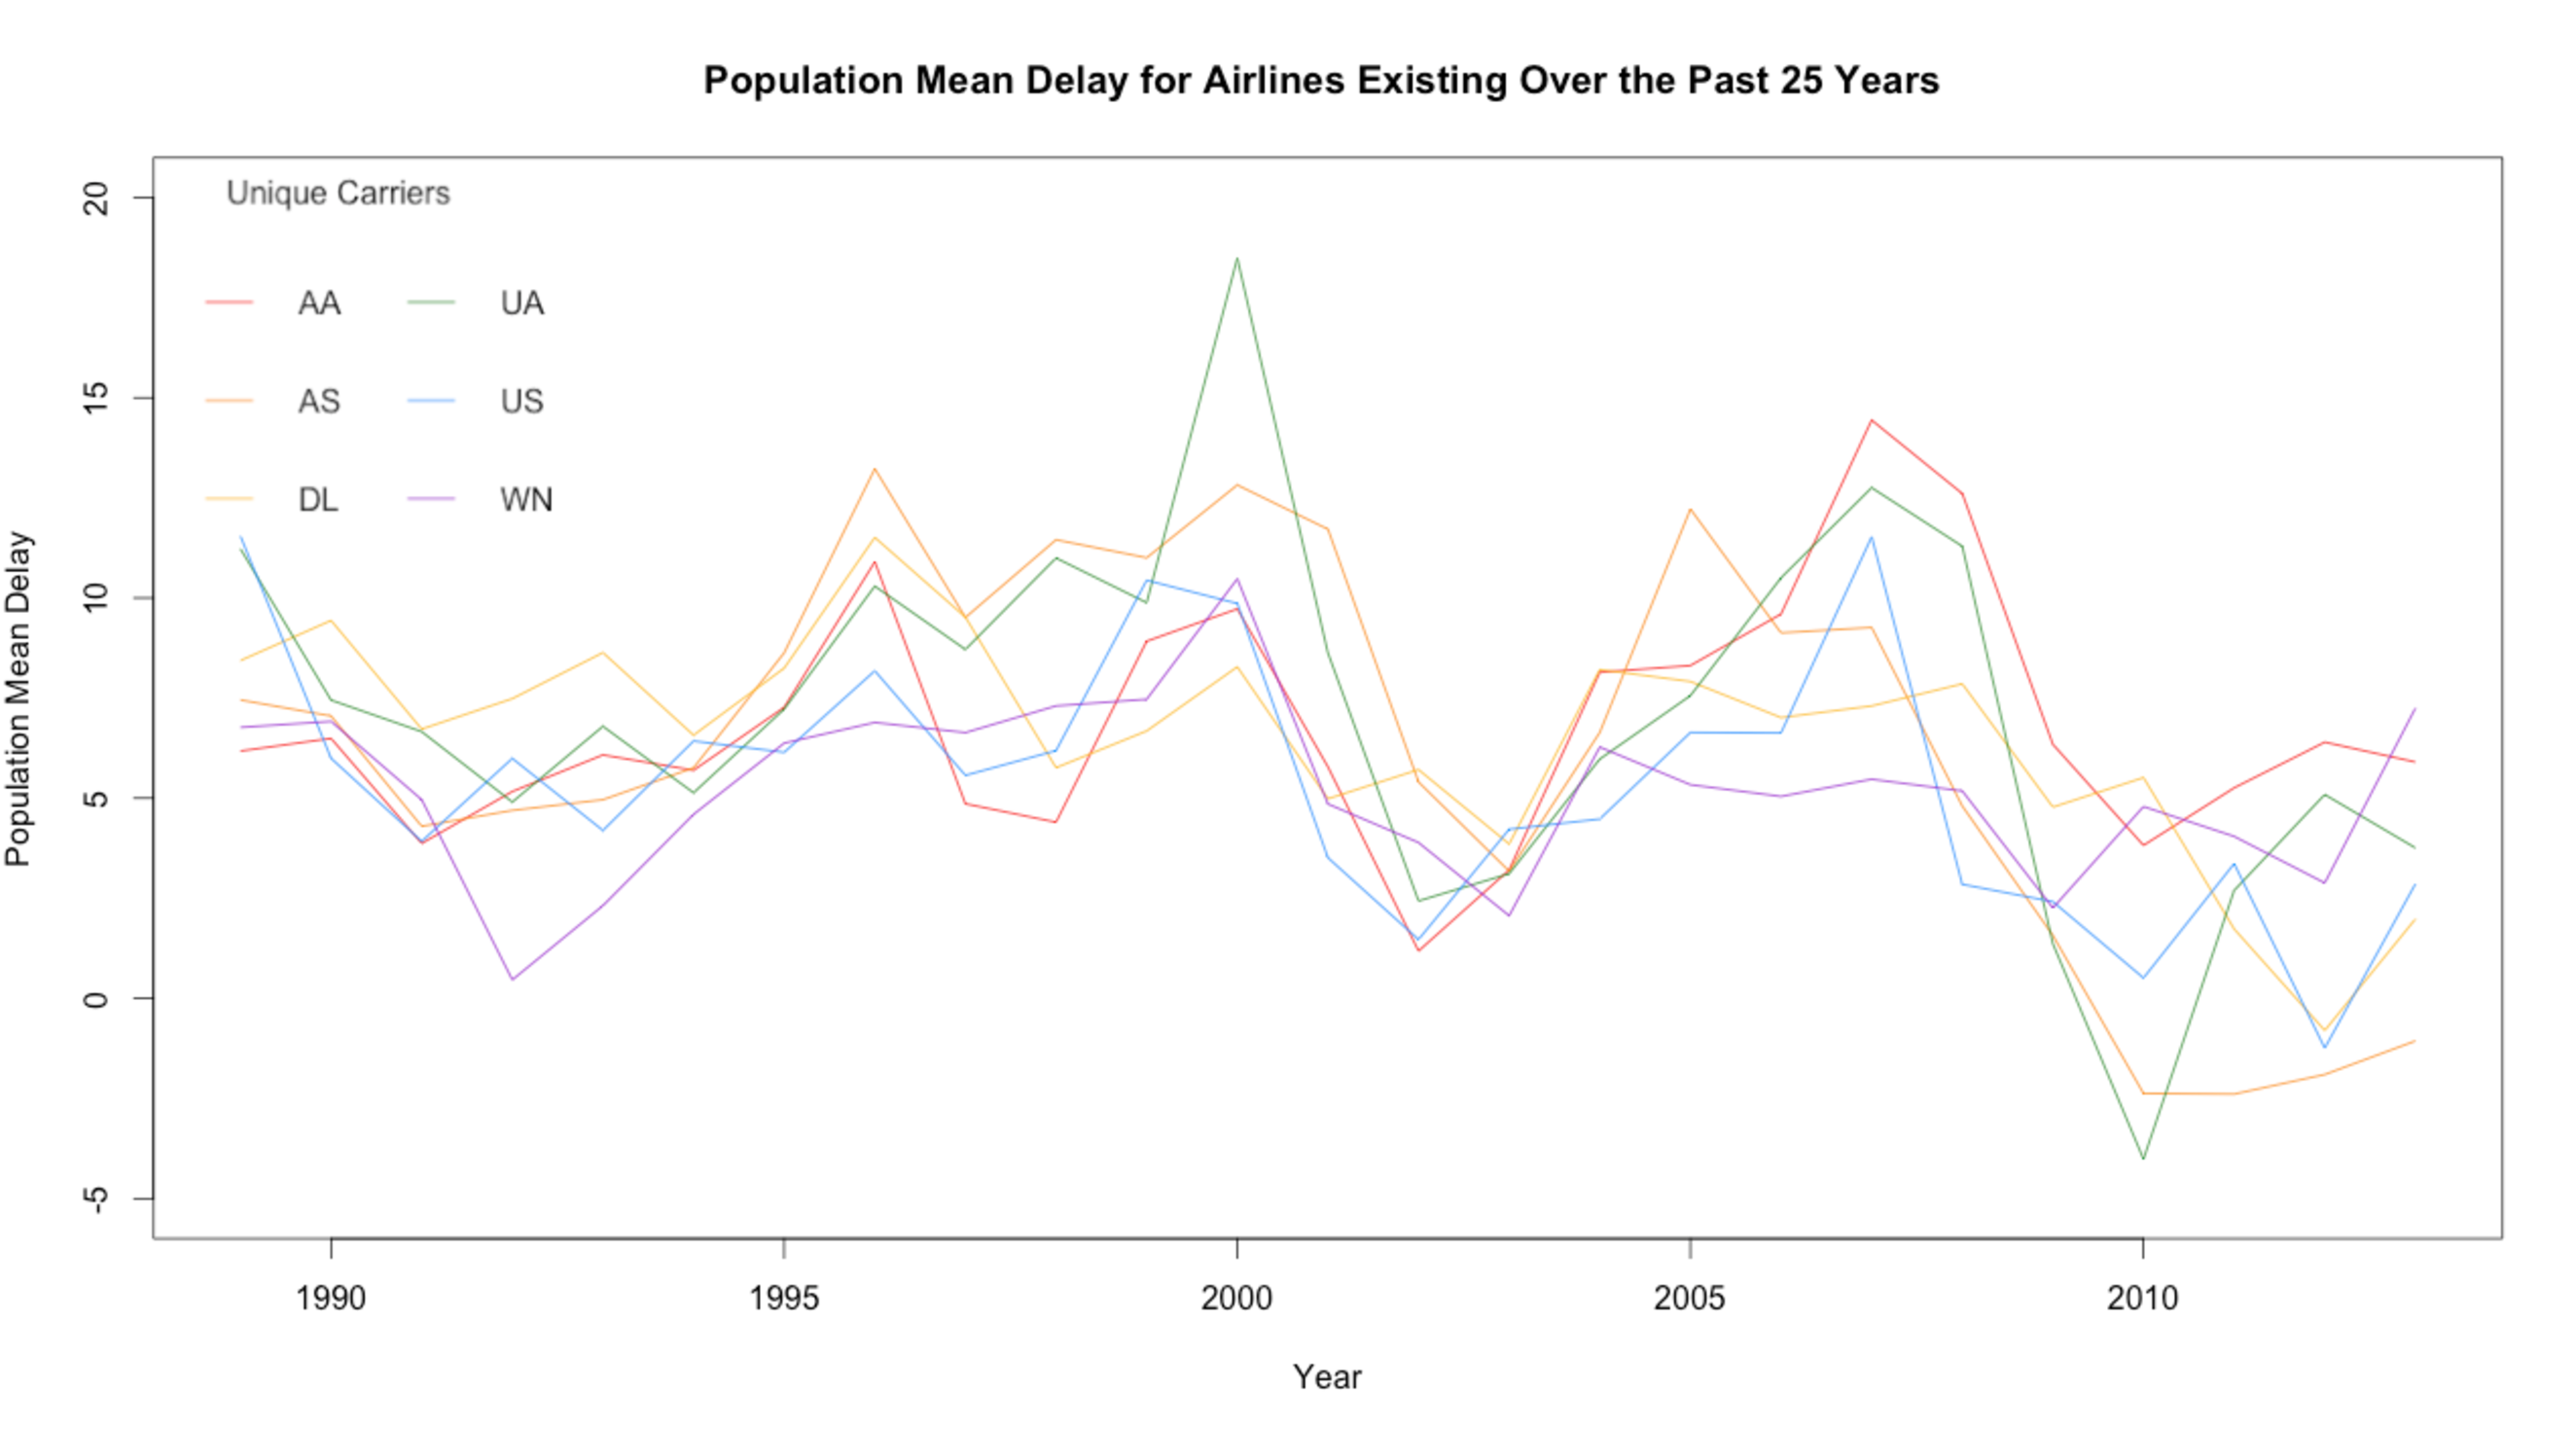
\includegraphics[width=1 \textwidth]{popMean}
\end{center}

\end{frame}

\begin{frame}
\frametitle{Population-Based Findings}
\begin{center} 
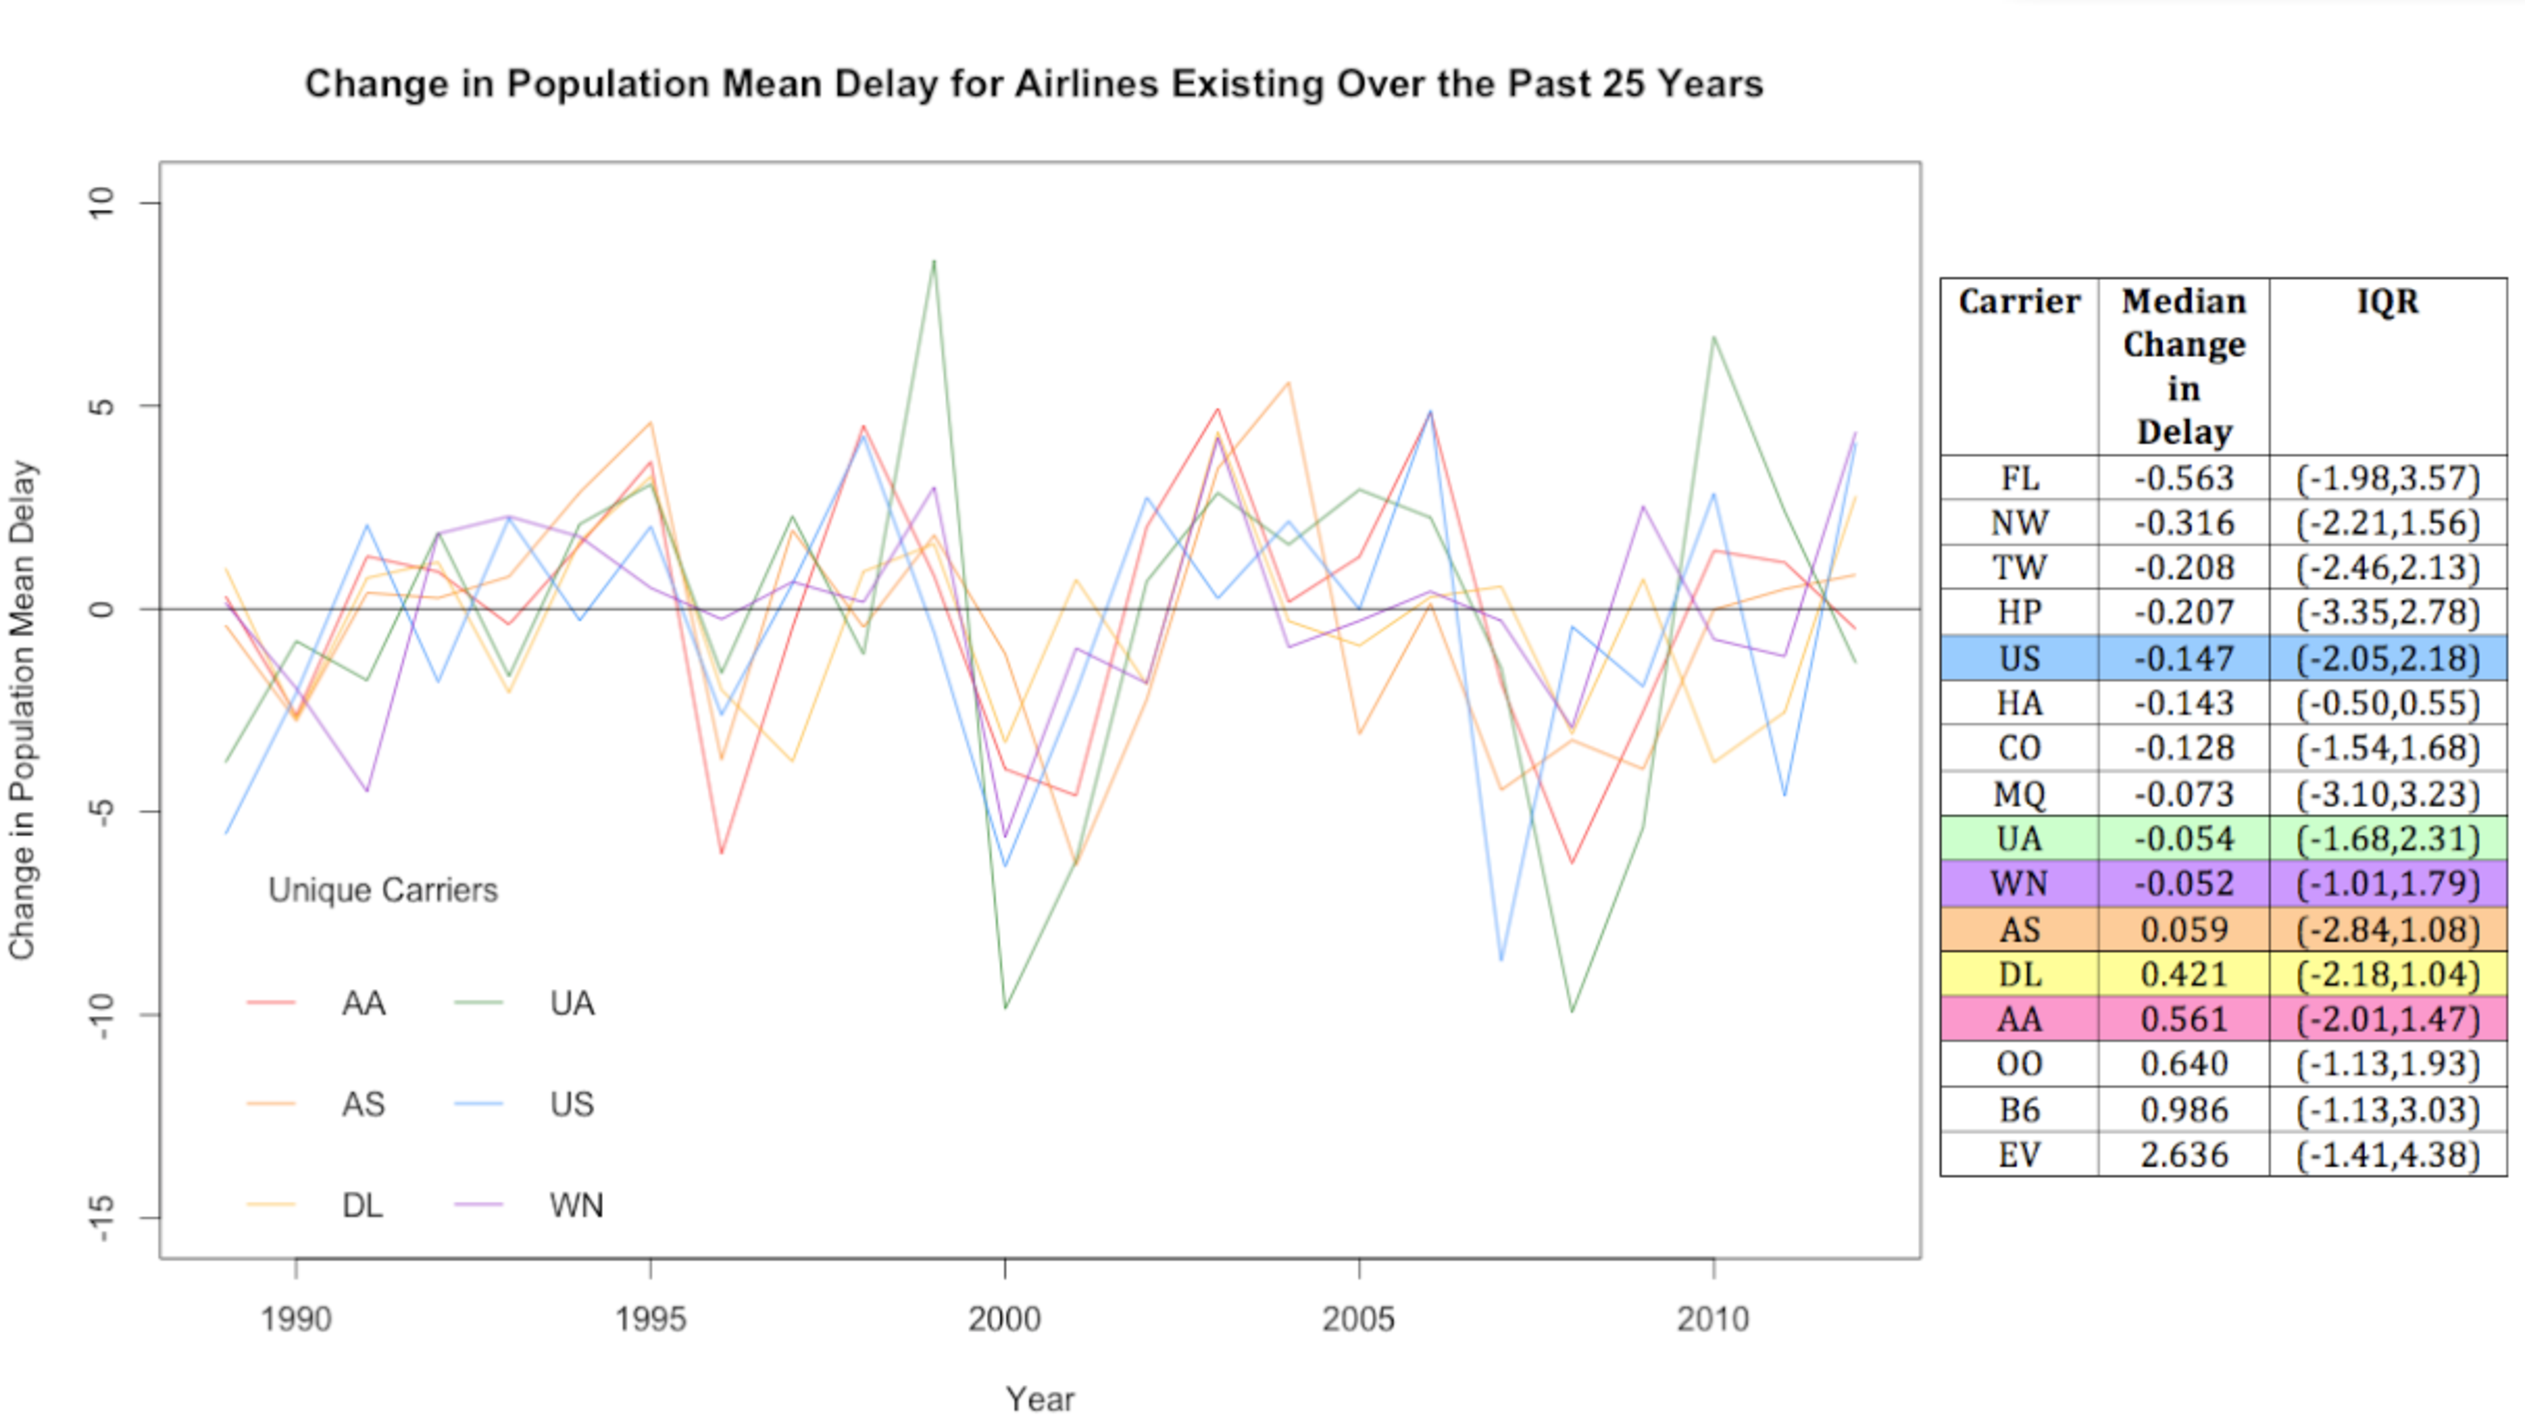
\includegraphics[width=1 \textwidth]{popPlot}
\end{center}

\end{frame}

\subsection{Patterns}
\begin{frame}
\frametitle{Patterns}
\begin{itemize}
\item Late 90's overall increase
\item Spike at 2000: possible 9/11
\item Decrease at 2003-2004
\item Steadily increased until 2007 
\begin{itemize}
\item Rising jet fuel prices 
\item Great Recession 
\end{itemize}
\end{itemize}

\end{frame}

\section{Sample-based Findings}
\begin{frame}
\frametitle{Sample-based Findings}
\begin{enumerate}
\item Stratify by unique carrier
\item Stratify by year (1989-2013)
\item Stratify by origin airport size 

(as determined by flight traffic volume)
\begin{itemize}
\item Proportional sample from strata based on number of flights 
\end{itemize}
\end{enumerate}

\end{frame}

\subsection{Sample Frame}
\begin{frame}
\frametitle{Sample Frame}
Assumption: Due to coordination of air traffic control efforts, flights originating from airports of similar traffic volume would have similarities in delay patterns
\begin{itemize}
\item Found traffic volume for each origin over 25 years 
\item Found average traffic volume 
\item Ordered and stratified based on size
\begin{itemize}
\item Create subsets of carriers 
\item Used $\%in\%$ when filtering
\end{itemize}
\end{itemize}
\end{frame}

\subsection{Findings}
\begin{frame}
\frametitle{Sample Findings}
\begin{center} 
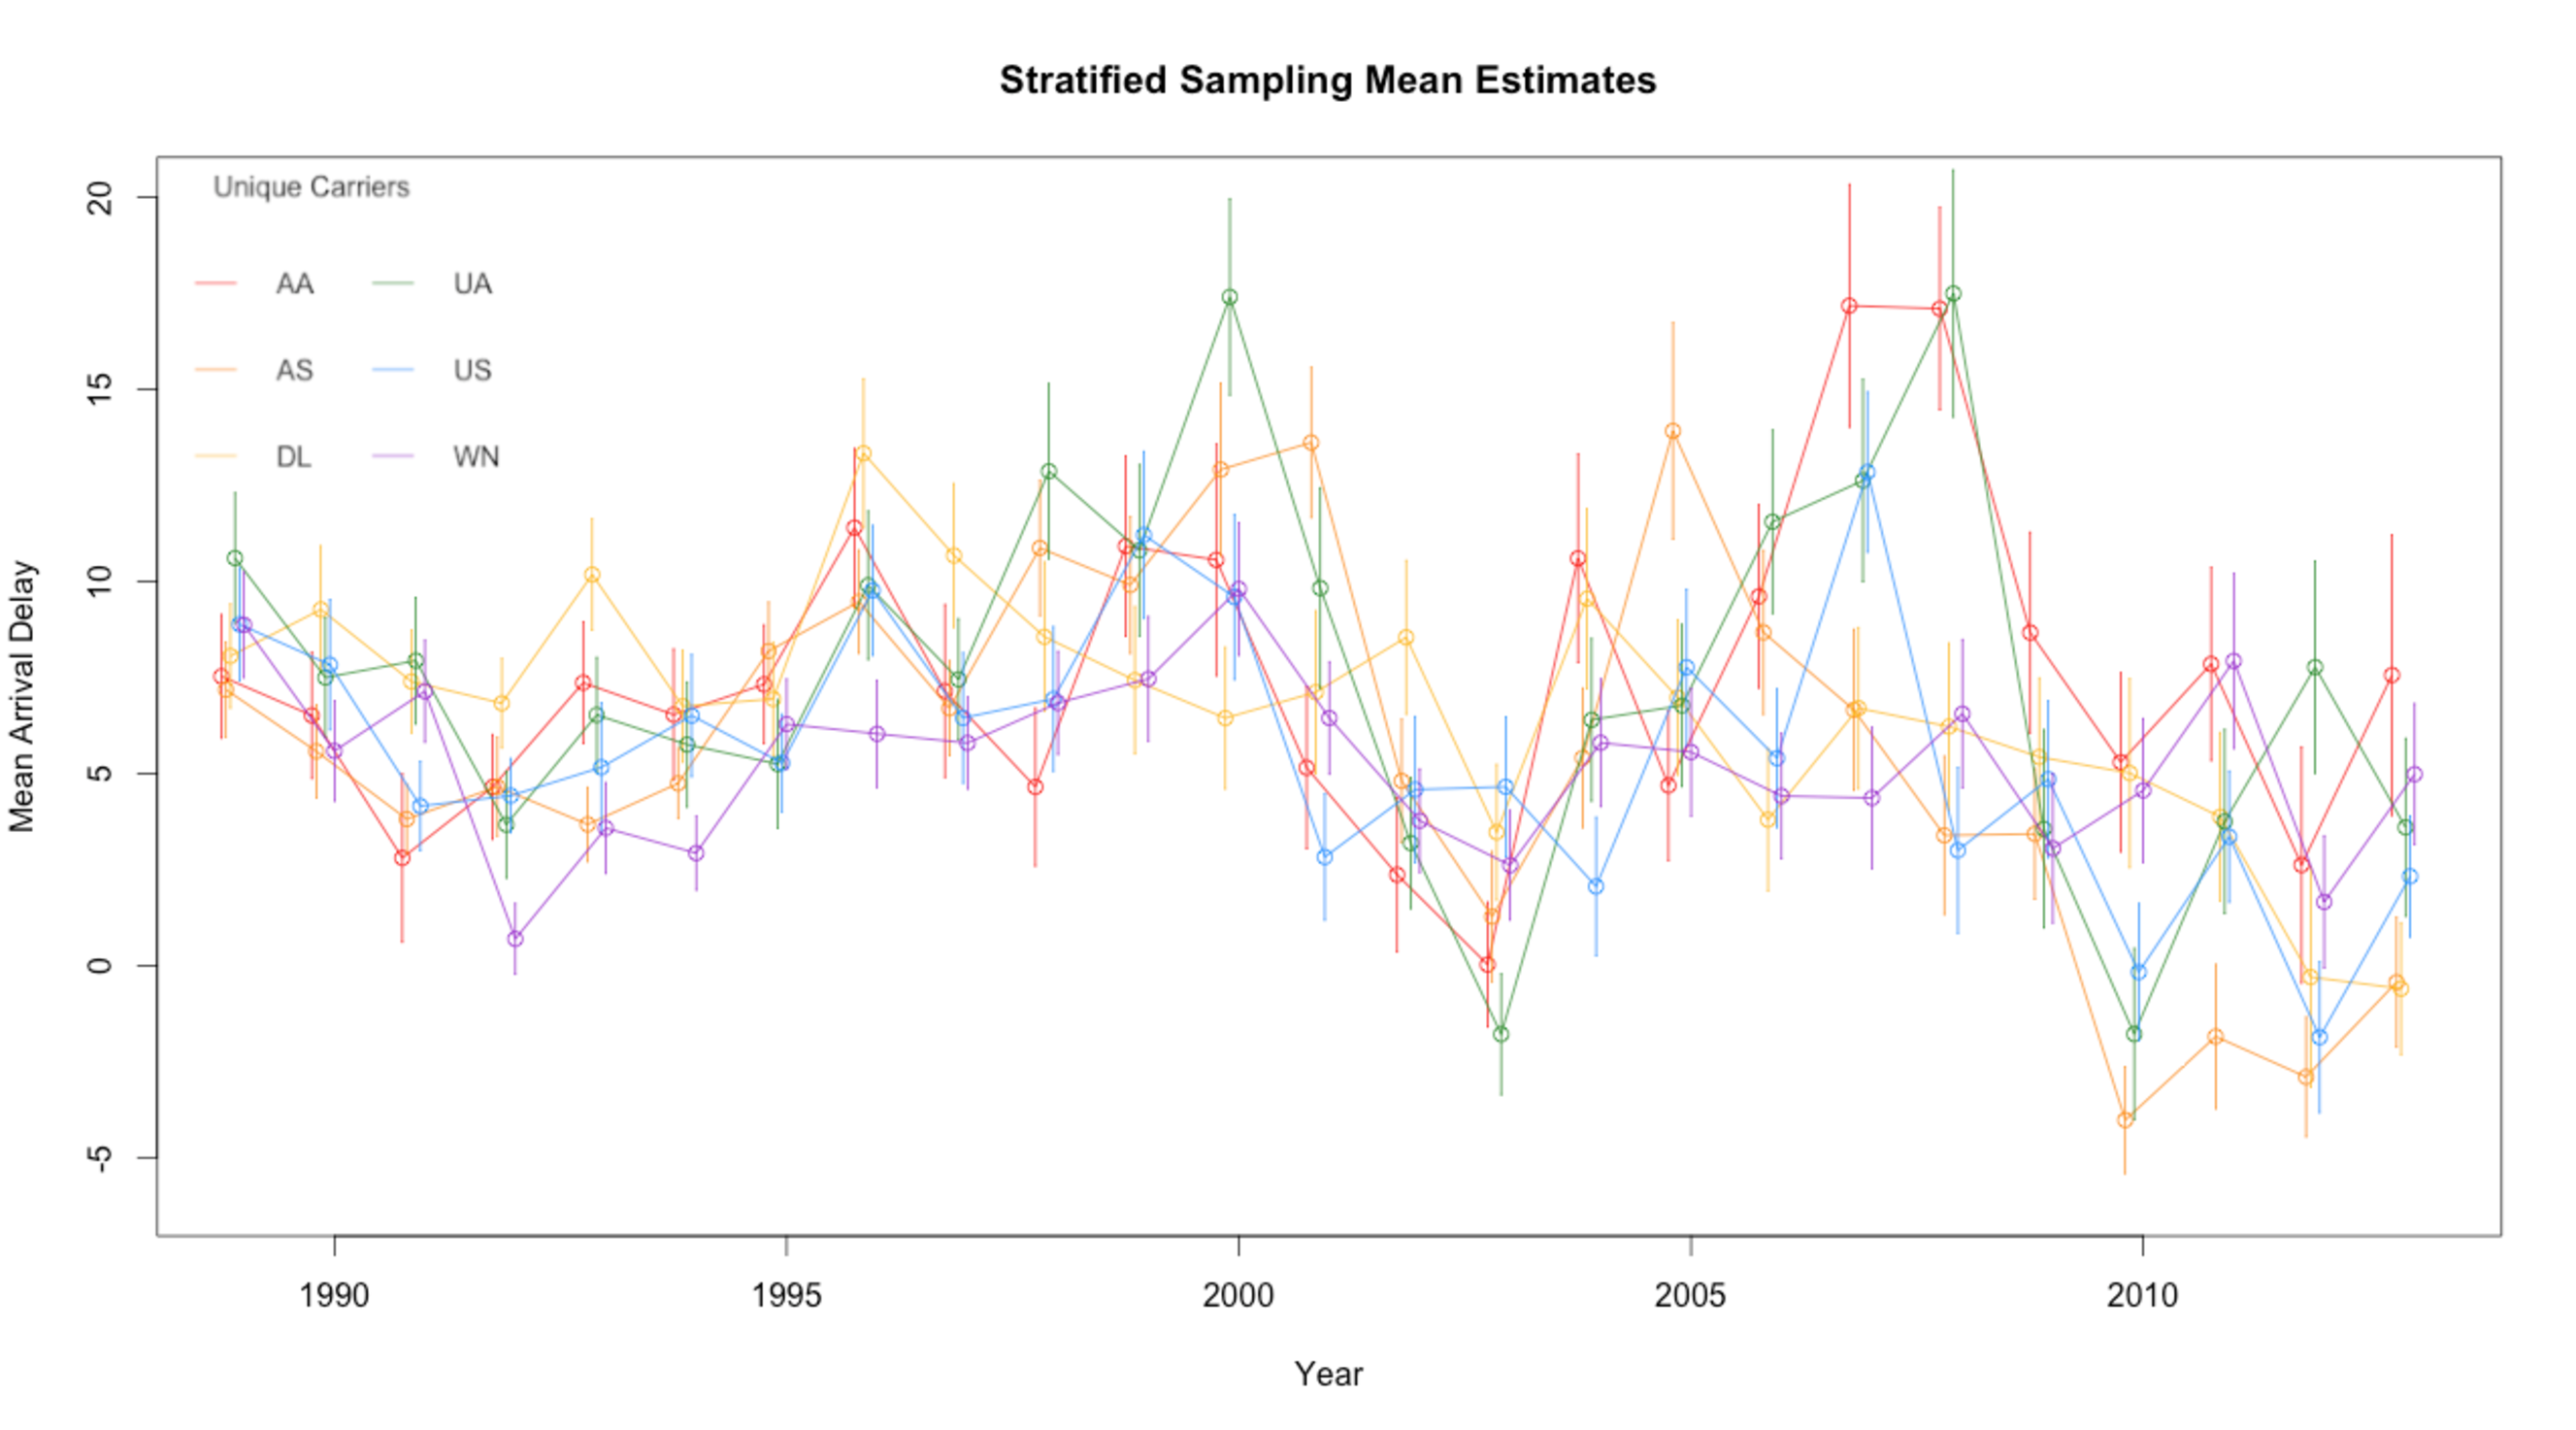
\includegraphics[width=1 \textwidth]{stratSampWithSE}
\end{center}

\end{frame}

\begin{frame}
\frametitle{Sample Findings}
\begin{center} 
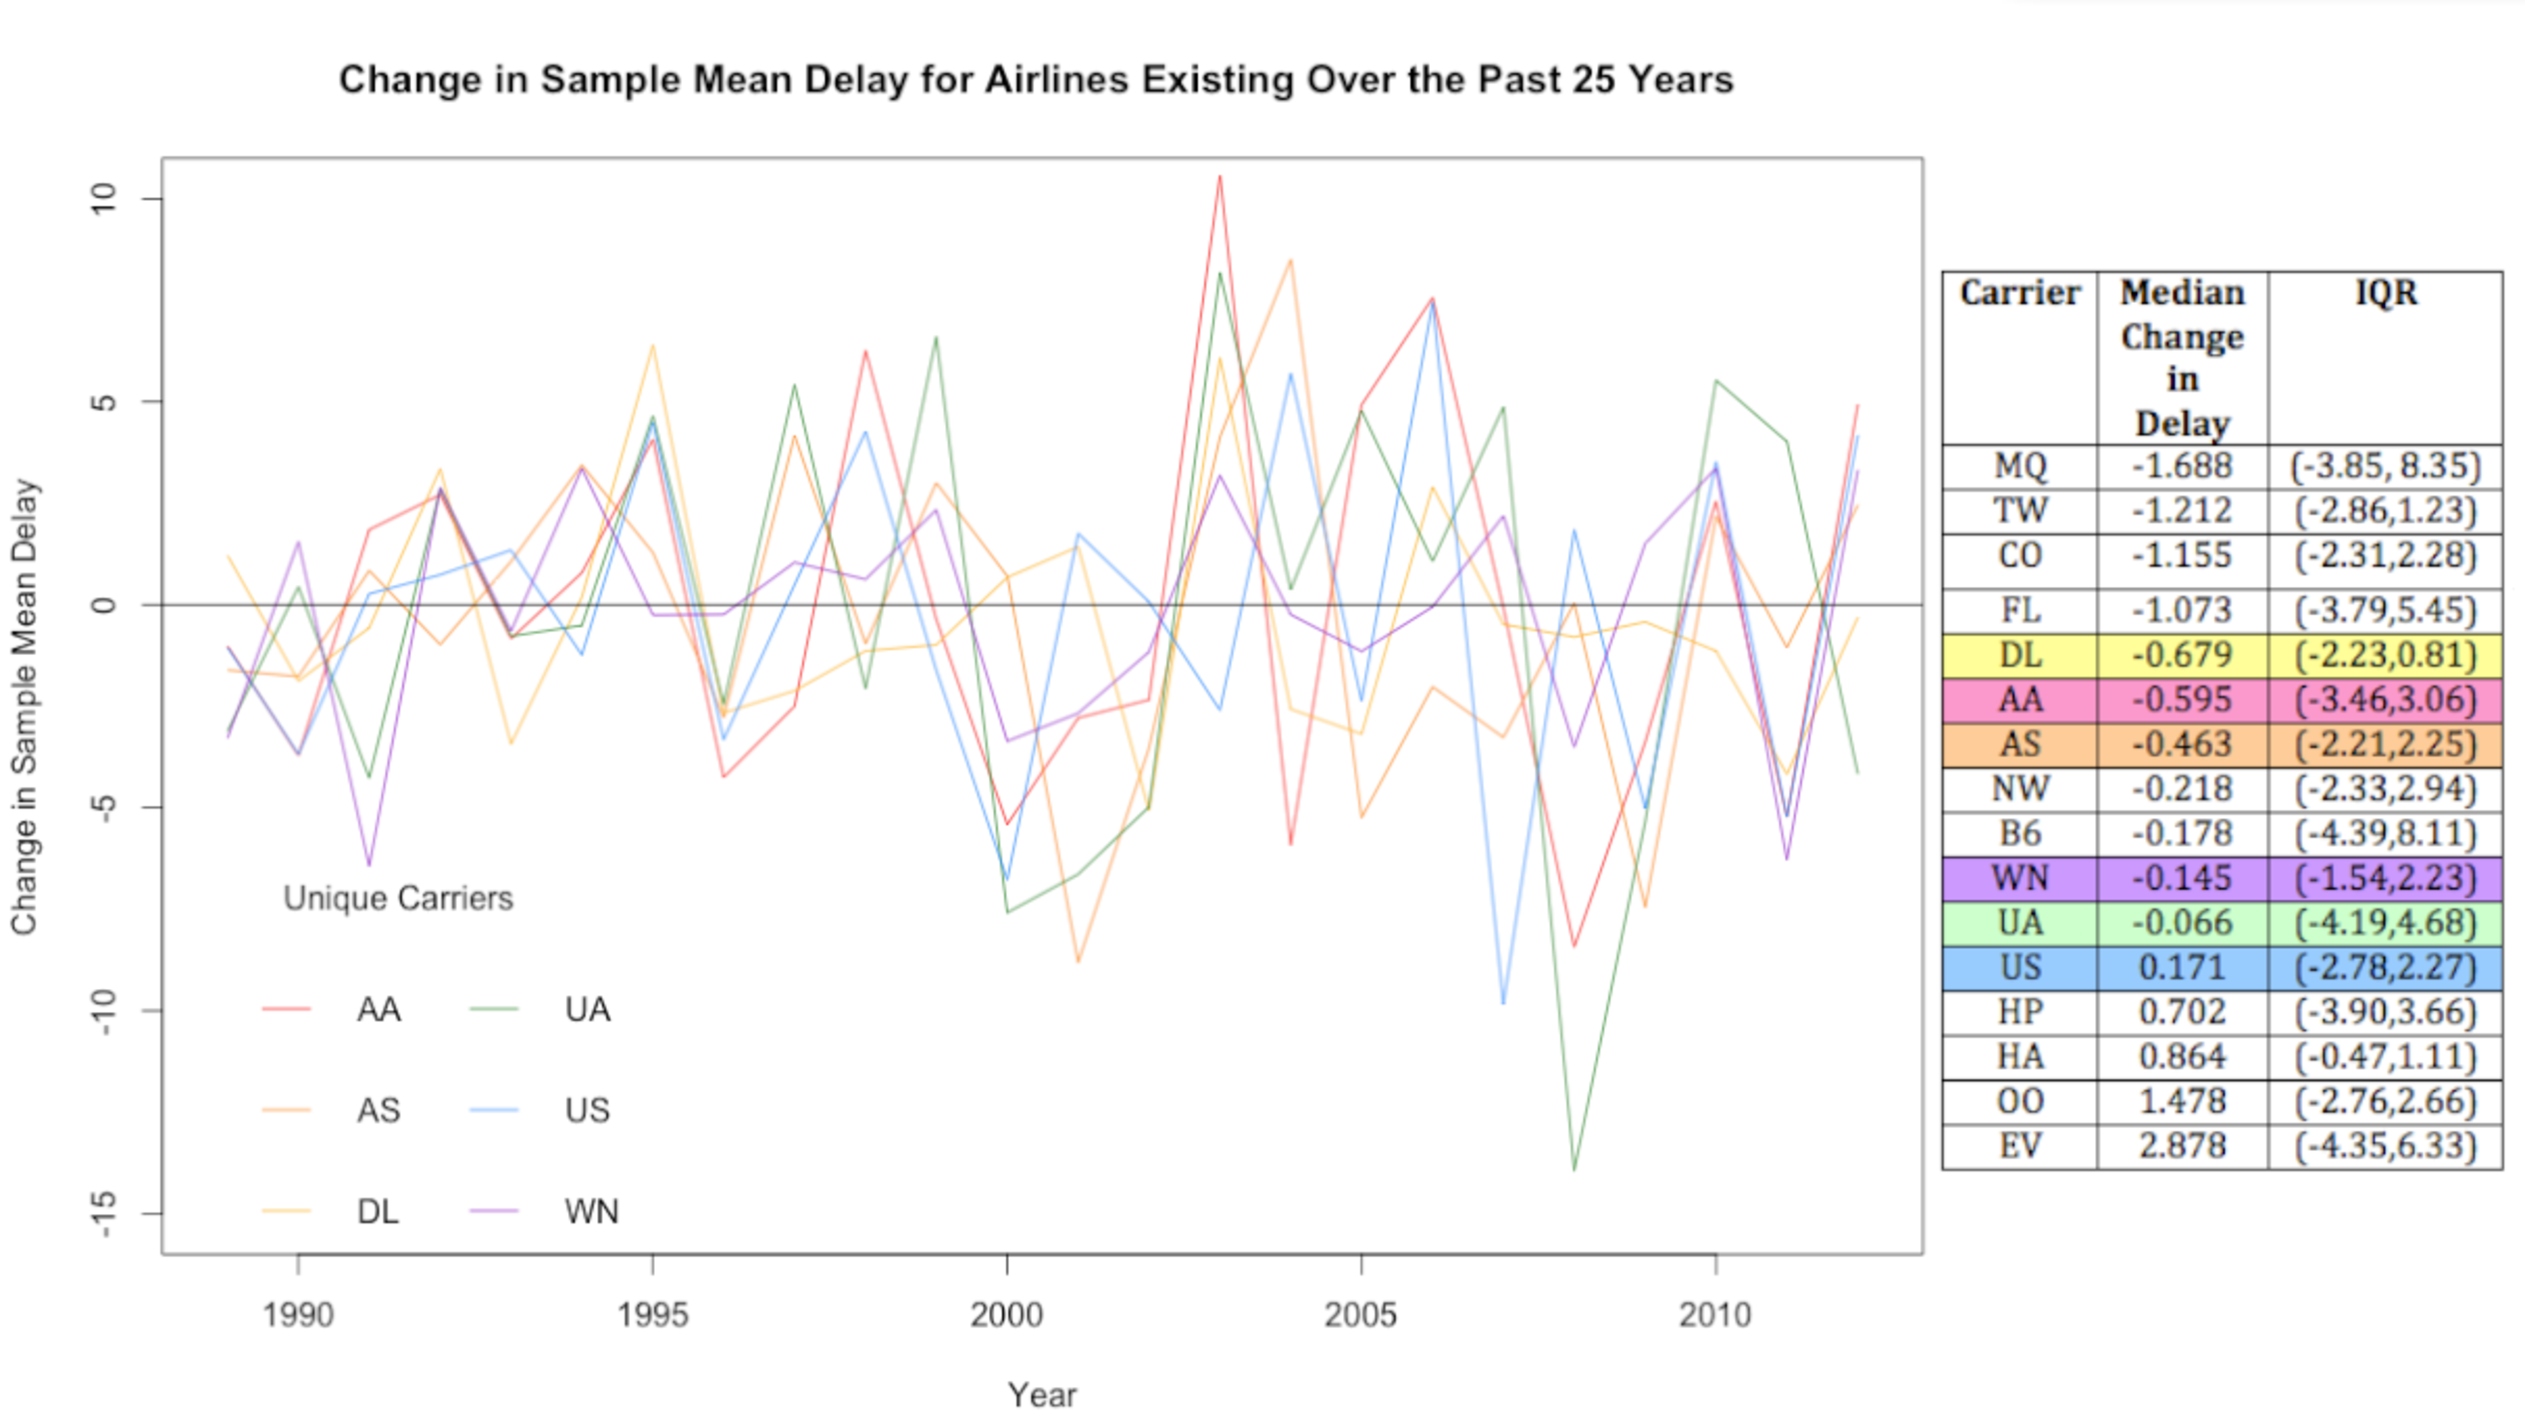
\includegraphics[width=1 \textwidth]{summarySamp}
\end{center}

\end{frame}



\subsection{Sampling Performance}
\begin{frame}
\frametitle{Sampling Performance: 76\% Coverage}
\begin{center} 
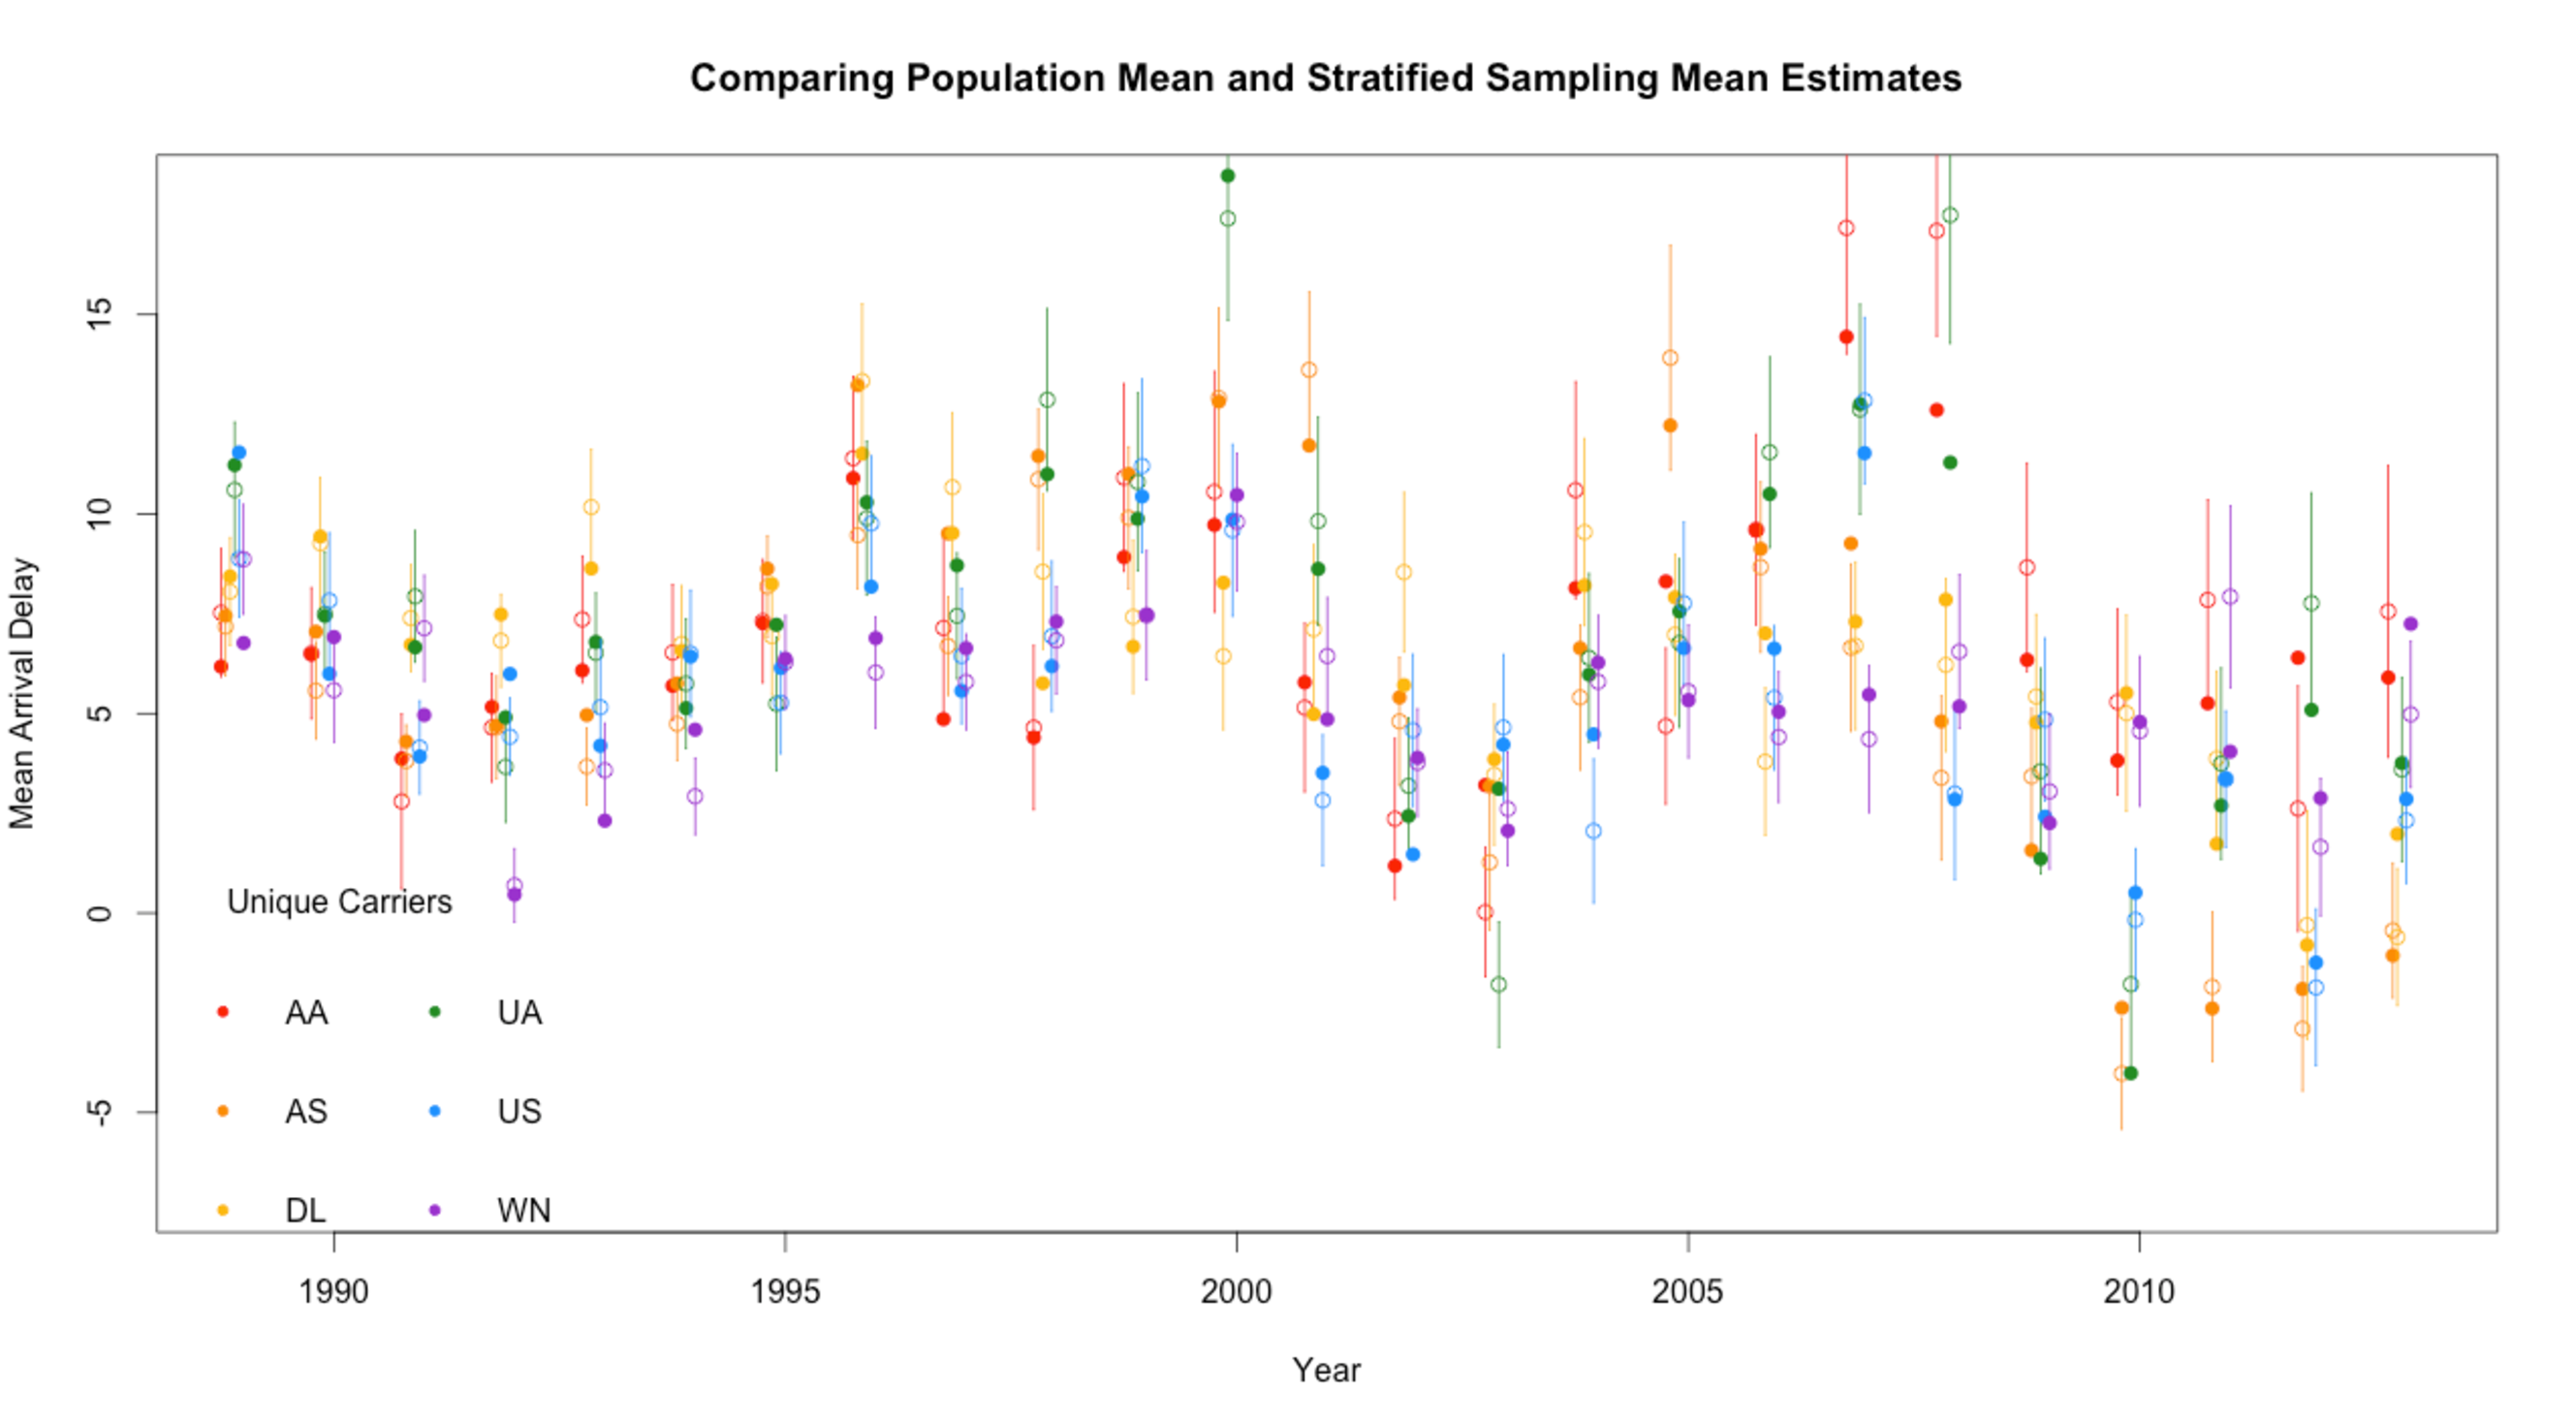
\includegraphics[width=1 \textwidth]{noLine}
\end{center}

\end{frame}

\begin{frame}
\frametitle{Bias}
\begin{center} 
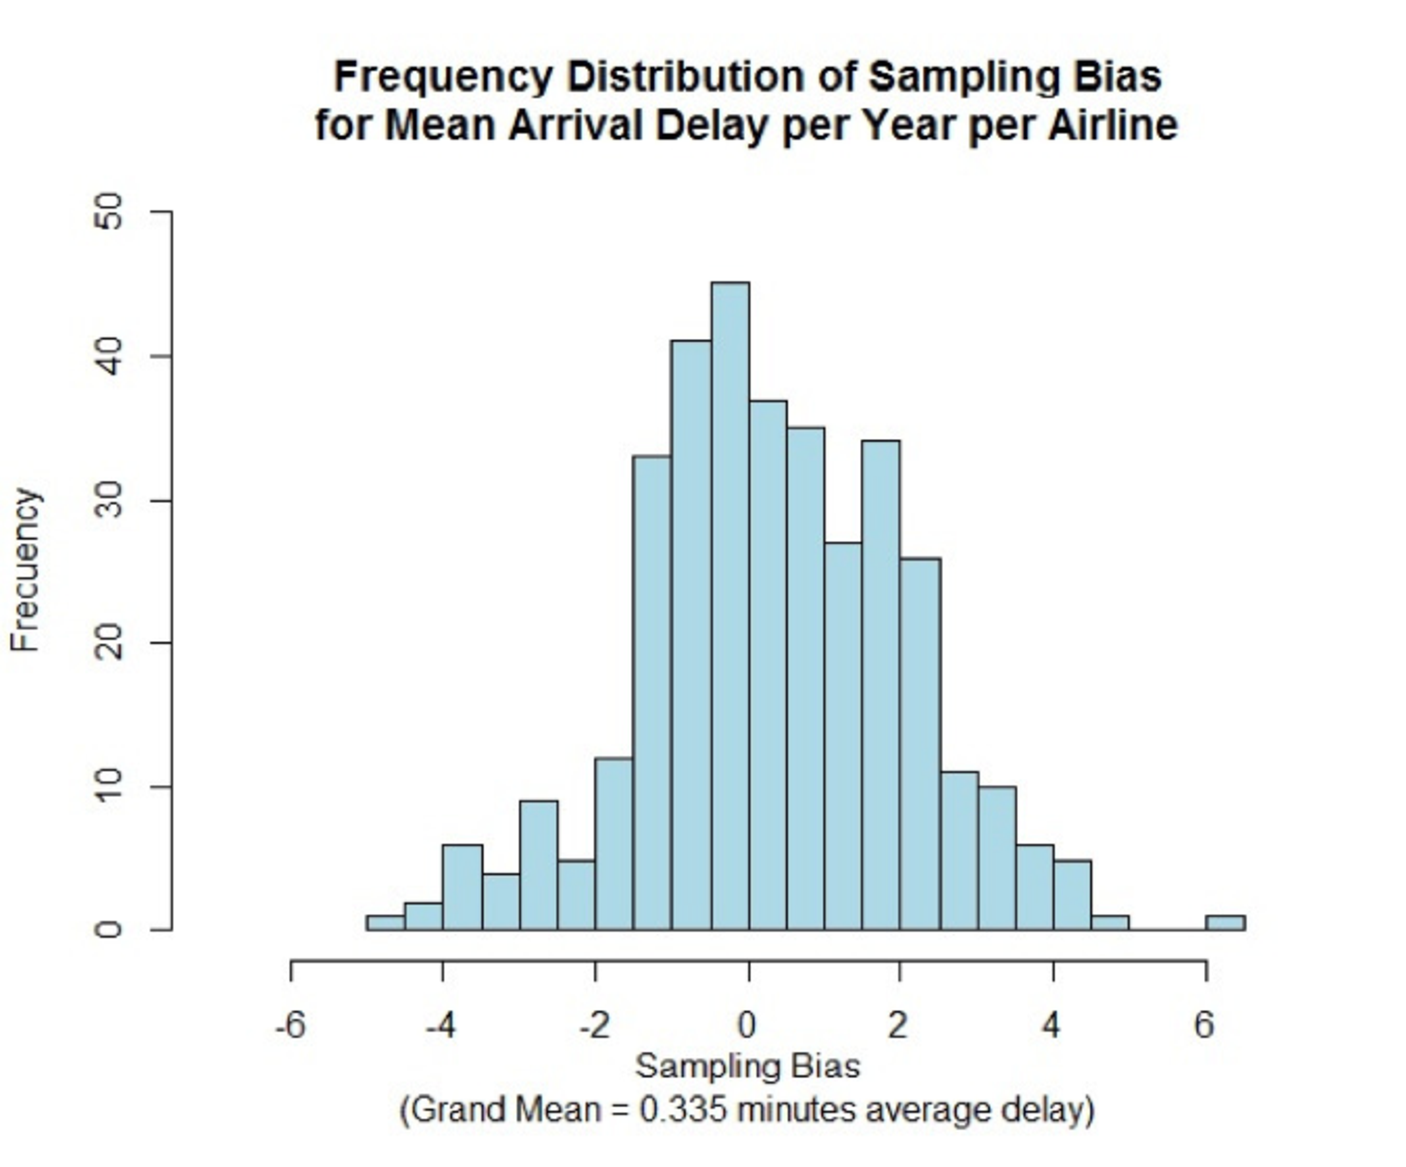
\includegraphics[width=.7 \textwidth]{bias}
\end{center}

\end{frame}


\section{Discussion, Obstacles and Solutions}
\begin{frame}
\frametitle{The "Simple" Answer}
\begin{itemize}
\item No, no one airline carrier is \emph{consistently} improving.
\item Nor did one airline carrier show \emph{consistent} improvement above all others. 
\end{itemize}

\end{frame}

\subsection{Cognitive Time vs Computational Time}
\begin{frame}
\frametitle{Cognitive Time vs Computational Time}
\begin{itemize}
\item Population Summary: ~6m 25s
\item Sample Summary: ~5.5 hrs 
\begin{itemize}
\item Sampling and collecting is slow 
\item Originally had stratified by airport origins 
\item Took 2.5 hours to sample from American Airlines in 1989
\end{itemize}
\end{itemize}

\end{frame}

\subsection{Data Visualization}
\begin{frame}
\frametitle{Data Visualization}
\begin{itemize}
\item Combating "spaghetti" plots
\item Ploting changes in mean delays 
\begin{itemize}
\item Think of this as the derivative 
\end{itemize}
\end{itemize}

\end{frame}

\section{Future Work}
\begin{frame}
\frametitle{Future Work}
\begin{itemize}
\item Understanding reasons for delay: 
\begin{itemize}
\item Comparing sources of delay that carriers can't control with sources of delay that carriers do control 
\end{itemize}
\item How one flight arriving late affect its subsequent stops? 
\item More specific strata, with access to higher computational resources / computation time
\end{itemize}

\end{frame}

\section{Questions}
\begin{frame}
\frametitle{Questions}
\begin{center}
\emph{Google? Which airline is sexy?}
\end{center}



\end{frame}

%\begin{center} 
%\includegraphics[width=1 \textwidth]{fieldmap}
%\end{center}
 






\end{document}